\section*{Problem 2}

Give a chip design containing three power components and eight regular components satisfying the following constraints:
\begin{itemize}
  \item The width of the chip is 29 and the height is 22.
  \item All power components have width 4 and height 2.
  \item The sizes of the eight regular components are $9 \times 7$, $12 \times 6$, $10 \times 7$, $18 \times 5$, $20 \times 4$, $10 \times 6$, $8 \times 6$ and $10 \times 8$, respectively.
  \item All components may be turned 90, but may not overlap.
  \item In order to get power, all regular components should directly be connected to a power component, that is, an edge of the component should have at least one point in common with an edge of the power component.
  \item Due to limits on heat production the power components should be not too close: their centres should differ at least 17 in either the $x$ direction or the $y$ direction (or both).
\end{itemize}

\vspace{4mm}

\subsection*{Solution:}
First of all, we assume the chip plan is a positive plane whose left-bottom corner has coordinate $(0, 0)$, and right-top corner has coordinate $(29, 22)$.
Next, we introduce coordinates to each corner of each components $(x_{ij}, y_{ij})$ to specify them.
See below.

\begin{enumerate}
  \item For the three power components:\\
  Power component 1 has coordinates $(x_{11}, y_{11})$, $(x_{12}, y_{11})$, $(x_{12}, y_{11})$ and $(x_{12}, y_{12})$.\\
  Power component 2 has coordinates $(x_{21}, y_{21})$, $(x_{22}, y_{21})$, $(x_{22}, y_{21})$ and $(x_{22}, y_{22})$.\\
  Power component 3 has coordinates $(x_{31}, y_{31})$, $(x_{32}, y_{31})$, $(x_{32}, y_{31})$ and $(x_{32}, y_{32})$.
  \item For the eight regular components:\\
  Regular component 1 has coordinates $(n_{11}, m_{11})$, $(n_{12}, m_{11})$, $(n_{12}, m_{11})$ and $(n_{12}, m_{12})$.\\
  Regular component 2 has coordinates $(n_{21}, m_{21})$, $(n_{22}, m_{21})$, $(n_{22}, m_{21})$ and $(n_{22}, m_{22})$.

  $\cdots \cdots$

  Regular component 8 has coordinates $(n_{81}, m_{81})$, $(n_{82}, m_{81})$, $(n_{82}, m_{81})$ and $(n_{82}, m_{82})$.
\end{enumerate}
Thus, we plan to put the components onto the plan in terms of the constraints.

\begin{description}
  \item[Constraint 1:] Now the chip is a positive plane, so all the coordinates should be positive. The width of the chip is 29 and the height is 22.

  Then we have
  \[  \bigwedge_{i=1}^3 29 \geq x_{i2} \geq x_{i1} \geq 0 \wedge 22 \geq y_{i2} \geq y_{i1} \geq 0 \;\; \wedge \]
  \[  \bigwedge_{i=1}^8 29 \geq n_{i2} \geq n_{i1} \geq 0 \wedge 22 \geq m_{i2} \geq m_{i1} \geq 0 \]
  \item[Constraint 2:] All power components have width 4 and height 2,
  and the sizes of the eight regular components are $9 \times 7$, $12 \times 6$, $10 \times 7$, $18 \times 5$, $20 \times 4$, $10 \times 6$, $8 \times 6$ and $10 \times 8$, respectively.
  All components may be turned 90.

  Then we have
  \[  \bigwedge_{i=1}^3 ((x_{i2} - x_{i1} = 4 \; \wedge \; y_{i2} - y_{i1} = 2) \;\; \vee \]
  \[ (x_{i2} - x_{i1} = 2 \; \wedge \; y_{i2} - y_{i1} = 4)) \]
  So do the coordinates for the Regular components. However their sizes are distinct,
  this makes more writing and coding. Here we only show the clause for the first regular component,
  whose size is $9 \times 7$. \\
  \[ (n_{12} - n_{11} = 9 \; \wedge \; m_{12} - m_{11} = 7) \;\; \vee (n_{12} - n_{11} = 7 \; \wedge \; m_{12} - m_{11} = 9) \]
  \item[Constraint 3:] All components may not overlap.

\begin{center}
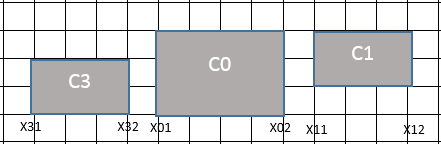
\includegraphics[width=0.5\textwidth]{Part1_2_1.png}
\end{center}
  As the figure shows, only if a component's $x_{i1}$ is larger than the other one's $x_{k2}$, then these two components are not overlapped. We also have the case in the y direction.

  Among the power components:

  \[  \bigwedge_{i,k: 1 \leq i \leq 3, 1 \leq k \leq 3, i \neq k}
  x_{i2} \leq x_{k1} \; \vee \; x_{k2} \leq x_{i1} \; \vee \; y_{i2} \leq y_{k1} \; \vee \; y_{k2} \leq y_{i1} \]

  Among the regular components:

  \[  \bigwedge_{i,k: 1 \leq i \leq 8, 1 \leq k \leq 8, i \neq k}
  n_{i2} \leq n_{k1} \; \vee \; n_{k2} \leq n_{i1} \; \vee \; m_{i2} \leq m_{k1} \; \vee \; m_{k2} \leq m_{i1}  \]

  Between the power components and the regular components:

  \[  \bigwedge_{i,k: 1 \leq i \leq 3, 1 \leq k \leq 8, i \neq k}
   x_{i2} \leq n_{k1} \; \vee \; n_{k2} \leq x_{i1} \; \vee \; y_{i2} \leq m_{k1} \; \vee \; m_{k2} \leq y_{i1} \]

  \item[Constraint 4:] An edge of the regular component should have at least one point in common with an edge of the power component.

\begin{center}
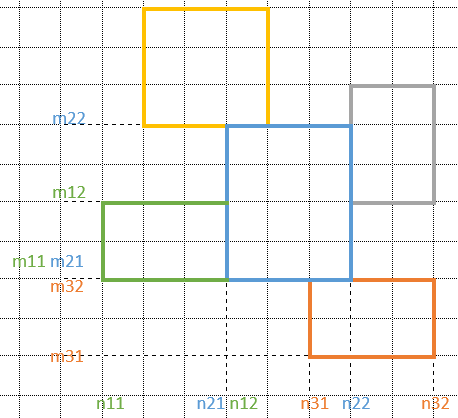
\includegraphics[width=0.5\textwidth]{Part1_2_2.png}
\end{center}

  As the figure above shows, if two components are touched at least one point, then at least one coordinate of a component is the same as the other one. We consider it from the inverse way to make the clauses simpler. If two components have the same $x_{i1}$ value, only if their $y$-direction sides are not touched, then these two components are not in common with an edge of each other.
  We denote this condition as follows.

  \[  \bigwedge_{i,k: 1 \leq i \leq 3, 1 \leq k \leq 8}
  ((x_{i2} = n_{k1} \; \vee \; x_{i1} = n_{k2}) \; \wedge \;
  \neg (y_{i2} < m_{k1} \vee m_{k2} < y_{i1}) \; \vee \; \]
  \[  ((y_{i2} = m_{k1} \; \vee \; y_{i1} = m_{k2}) \; \wedge \;
  \neg (x_{i2} < n_{k1} \vee n_{k2} < x_{i1}))) \]
  \item[Constraint 5:] The power components' centres should differ at least 17 in either the $x$ direction or the $y$ direction (or both).

  The centers of the power components are $(x_{i1} + \frac{x_{i2} - x_{i1}}{2}, y_{i1} + \frac{y_{i2} - y_{i1}}{2} )$.

  For each pair of the power components, we have

  \[  \bigwedge_{i,k: 1 \leq i < k \leq 3}
  [ (x_{i1} + \frac{x_{i2} - x_{i1}}{2}) - (x_{k1} + \frac{x_{k2} - x_{k1}}{2}) \geq 17 \; \vee \; \]
  \[ (x_{k1} + \frac{x_{k2} - x_{k1}}{2}) - (x_{i1} + \frac{x_{i2} - x_{i1}}{2}) \geq 17 \; \vee \; \]
  \[ (y_{k1} + \frac{y_{k2} - y_{k1}}{2}) - (y_{i1} + \frac{y_{i2} - y_{i1}}{2}) \geq 17 \; \vee \; \]
  \[ (y_{i1} + \frac{y_{i2} - y_{i1}}{2}) - (y_{k1} + \frac{y_{k2} - y_{k1}}{2}) \geq 17 ] \]


\end{description}

Making a conjunction of all the clauses derived from the constraints, we made the Yices smt cods.

This formula is easily expressed in SMT syntax.

{\footnotesize

{\tt (benchmark Part1\_2.smt}

{\tt :logic $QF\_LIA$}

{\tt :extrafuns (}

{\tt (x11 Int) (x12 Int) (y11 Int) (y12 Int)}

{\tt (x21 Int) (x22 Int) (y21 Int) (y22 Int)}

{\tt (x31 Int) (x32 Int) (y31 Int) (y32 Int)}

{\tt (n11 Int) (n12 Int) (m11 Int) (m12 Int)}

{\tt (n21 Int) (n22 Int) (m21 Int) (m22 Int)}

$\cdots \cdots$

{\tt (n81 Int) (n82 Int) (m81 Int) (m82 Int)}

{\tt )}

{\tt :formula (and}

{\tt (>= 29 x12) (>= x12 x11) (>= x11 0) (>= 22 y12) (>= y12 y11) (>= y11 0)}

{\tt (>= 29 x22) (>= x22 x21) (>= x21 0) (>= 22 y22) (>= y22 y21) (>= y21 0)}

{\tt (>= 29 x32) (>= x32 x31) (>= x31 0) (>= 22 y32) (>= y32 y31) (>= y31 0)}

{\tt (>= 29 n12) (>= n12 n11) (>= n11 0) (>= 22 m12) (>= m12 m11) (>= m11 0)}

{\tt (>= 29 n22) (>= n22 n21) (>= n21 0) (>= 22 m22) (>= m22 m21) (>= m21 0)}

$\cdots \cdots$

{\tt (>= 29 n82) (>= n82 n81) (>= n81 0) (>= 22 m82) (>= m82 m81) (>= m81 0)}

{\tt (or (and (>= 29 x12) (>= 22 y12) (= (- x12 x11) 4) (= (- y12 y11) 2))}

{\tt (and (>= 22 x12) (>= 29 y12) (= (- y12 y11) 4) (= (- x12 x11) 2)))}

$\cdots \cdots$

{\tt (or (and (= (- x32 x31) 4) (= (- y32 y31) 2)) (and (= (- x32 x31) 2) (= (- y32 y31) 4)))}

{\tt (or (and (= (- n12 n11) 9) (= (- m12 m11) 7)) (and (= (- n12 n11) 7) (= (- m12 m11) 9)))}

$\cdots \cdots$

{\tt (or (and (= (- n82 n81) 10) (= (- m82 m81) 8)) (and (= (- n82 n81) 8) (= (- m82 m81) 10)))}

{\tt ;; not overlap among power components}

{\tt (or (<= x12 x21) (<= x22 x11) (<= y12 y21) (<= y22 y11))}

{\tt (or (<= x12 x31) (<= x32 x11) (<= y12 y31) (<= y32 y11))}

{\tt (or (<= x32 x21) (<= x22 x31) (<= y32 y21) (<= y22 y31))}

{\tt ;; not overlap among regular components}

{\tt (or (<= n12 n21) (<= n22 n11) (<= m12 m21) (<= m22 m11))}

{\tt (or (<= n12 n31) (<= n32 n11) (<= m12 m31) (<= m32 m11))}

$\cdots \cdots$

{\tt (or (<= n72 n81) (<= n82 n71) (<= m72 m81) (<= m82 m71))}

{\tt ;;not overlap between power components and regular ones}

{\tt (or (<= x12 n11) (<= n12 x11) (<= y12 m11) (<= m12 y11))}

{\tt (or (<= x12 n21) (<= n22 x11) (<= y12 m21) (<= m22 y11))}

$\cdots \cdots$

{\tt (or (<= x32 n81) (<= n82 x31) (<= y32 m81) (<= m82 y31))}

{\tt ;;Constraint 4}

{\tt (or}

{\tt (and (or (= x11 n12) (= x12 n11)) (not (or (< y12 m11) (> y11 m12))))}

{\tt (and (or (= x21 n12) (= x22 n11)) (not (or (< y22 m11) (> y21 m12))))}

$\cdots \cdots$

{\tt (and (or (= y31 m12) (= y32 m11)) (not (or (< x32 n11) (> x31 n12))))}

{\tt )}

$\cdots \cdots$

{\tt (or}

{\tt (and (or (= x11 n82) (= x12 n81)) (not (or (< y12 m81) (> y11 m82))))}

{\tt (and (or (= x21 n82) (= x22 n81)) (not (or (< y22 m81) (> y21 m82))))}

$\cdots \cdots$

{\tt (and (or (= y31 m82) (= y32 m81)) (not (or (< x32 n81) (> x31 n82))))}

{\tt )}

{\tt ;;Constraint 5}

{\tt (or (>= (- (+ x11 (/ (- x12 x11) 2)) (+ x21 (/ (- x22 x21) 2))) 17)}

{\tt (>= (- (+ x21 (/ (- x22 x21) 2)) (+ x11 (/ (- x12 x11) 2))) 17)}

{\tt (>= (- (+ y11 (/ (- y12 y11) 2)) (+ y21 (/ (- y22 y21) 2))) 17)}

{\tt (>= (- (+ y21 (/ (- y22 y21) 2)) (+ y11 (/ (- y12 y11) 2))) 17))}

$\cdots \cdots$

{\tt (or (>= (- (+ x11 (/ (- x12 x11) 2)) (+ x31 (/ (- x32 x31) 2))) 17)}

{\tt (>= (- (+ x31 (/ (- x32 x31) 2)) (+ x11 (/ (- x12 x11) 2))) 17)}

{\tt (>= (- (+ y11 (/ (- y12 y11) 2)) (+ y31 (/ (- y32 y31) 2))) 17)}

{\tt (>= (- (+ y31 (/ (- y32 y31) 2)) (+ y11 (/ (- y12 y11) 2))) 17))}

{\tt ))}
}

Applying {\tt yices-smt -m part$1\_2$.smt}, we test out a satisfiable chip design plan.

{\footnotesize

{\tt sat}

{\tt(= x11 4)}

{\tt(= x12 6)}

{\tt(= y11 2)}

{\tt(= y12 6)}

{\tt(= x21 0)}

{\tt(= x22 4)}

{\tt(= y21 20)}

{\tt(= y22 22)}

{\tt(= x31 21)}

{\tt(= x32 23)}

{\tt(= y31 10)}

{\tt(= y32 14)}

{\tt(= n11 12)}

{\tt(= n12 21)}

{\tt(= m11 10)}

{\tt(= m12 17)}

{\tt(= n21 23)}

{\tt(= n22 29)}

{\tt(= m21 10)}

{\tt(= m22 22)}

{\tt(= n31 4)}

{\tt(= n32 22)}

{\tt(= m31 17)}

{\tt(= m32 22)}

{\tt(= n41 14)}

{\tt(= n42 21)}

{\tt(= m41 0)}

{\tt(= m42 10)}

{\tt(= n51 0)}

{\tt(= n52 4)}

{\tt(= m51 0)}

{\tt(= m52 20)}

{\tt(= n61 5)}

{\tt(= n62 11)}

{\tt(= m61 6)}

{\tt(= m62 16)}

{\tt(= n71 6)}

{\tt(= n72 14)}

{\tt(= m71 0)}

{\tt(= m72 6)}

{\tt(= n81 21)}

{\tt(= n82 29)}

{\tt(= m81 0)}

{\tt(= m82 10)}

}

\begin{center}
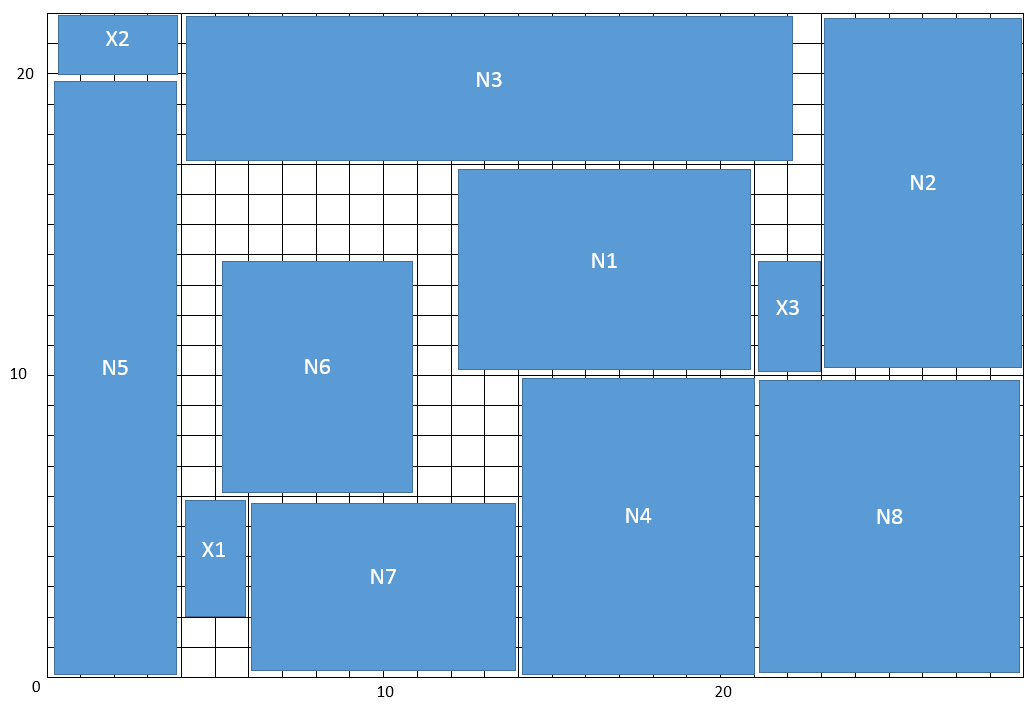
\includegraphics[width=0.8\textwidth]{Part1_2_3.png}
\end{center}

\subsection*{Remark:}

\subsection*{Generalization:}